\documentclass[12pt,a4paper]{article}
\usepackage{geometry}
\geometry{
	a4paper,
	total={170mm,257mm},
	left=20mm,
	top=20mm,
}
\usepackage{graphicx}
\usepackage{pdfpages}
\usepackage{float}
\usepackage{multirow}

\usepackage{polski}
\usepackage[utf8]{inputenc}

\begin{document}
	
	\begin{titlepage}
		\newgeometry{top=5.5cm, bottom=3cm}
		
		\centering
		{\huge\bfseries Technologie Sieciowe 2 - projekt\par}
		
		\vspace{0.5cm}
		Prowadzący: Dr inż. Wojciech Kmiecik (E02-88c, środa TP 9:15) \\
	
		\vspace{1.1cm}
		{\Large Dokumentacja projektu\par}
		\vspace{1.1cm}
		{\Large \bfseries Zestaw 12\par}
		\vfill
		
		{\large\bfseries Jakub Dorda 235013\par}
		{\large\bfseries Janusz Długosz 235746\par}
		{\large\bfseries Marcin Kotas 235098\par}
		
		\vspace{1cm}
		\today \\ \LaTeX
		
		\restoregeometry
	\end{titlepage}
	
	%wprowadzenie
	
	\tableofcontents
	\pagebreak
	
	\section{Wstęp - charakterystyka działalności instytucji}
	
	Celem projektu jest zaprojektowanie sieci komputerowej dla urzędu miejskiego. Instytucja posiada 3 wydziały zajmujące się	nieruchomościami, podatkami oraz pojazdami mechanicznymi. Na skutek zmian prawnych w kodeksie podatkowym oraz użytkowania wieczystego wystąpiła konieczność zatrudnienia większej ilości urzędników, więc zdecydowano o konieczności przeniesienia urzędu do większego budynku. Niestety gmina nie dysponowała odpowiednio dużym budynkiem, co poskutkowało koniecznością podziału urzędu na dwie nie połączone ze sobą części. Na skutek bezmyślnego oraz krótkowzrocznego zarządzania zasobami ludzkimi wszystkie działy zostały rozbite na poszczególne piętra wraz z filiami w drugim budynku. Nowy adres urzędu - ul. Kazimierza Wielkiego 29 we Wrocławiu.\\
	
	Projekt dotyczy wdrożenia sieci komputerowej w postaci zintegrowanego i jednolitego systemu informatycznego. Realizacja ma zapewniać rozwiązanie następujących problemów wynikających z wymagań projektu:
	\begin{itemize}
		\item wydziały są rozproszone po różnych piętrach i budynkach,
		\item łącze między budynkami jest ograniczone i nie podlega modyfikacji w projekcie,
		\item każdy dział wymaga stabilnego dostępu do sieci wewnętrznej oraz zewnętrznej,
		\item sieć wewnętrzna oraz dostęp do Internetu musi spełniać odpowiednie standardy bezpieczeństwa
	\end{itemize} 

	\noindent
	W ramach projektu przedstawione zostaną:
	 
	\begin{itemize}
		\item inwentaryzacja zasobów,
		\item analiza potrzeb użytkowników,
		\item założenia projektowe,
		\item projekt sieci,
		\item karty katalogowe proponowanych urządzeń 
	\end{itemize} 
	
	
	\section{Inwentaryzacja zasobów: sprzętu, aplikacji, zasobów ludzkich}
	Urząd jest podzielony na dwa osobne budynki oddalone od siebie o 320 $m$. Okablowanie między budynkami jest optyczne jednomodowe. Pierwszy z nich jest podzielony na 4 piętra, każdy z działów posiada pomieszczenia na każdym z nich. Drugi budynek ma jedno piętro również posiada filie każdego z wydziałów pierwszego budynku. Urząd na każdym piętrze korzysta z drukarek sieciowych, w sumie z 8. Na piętrze 2 i 4 budynku pierwszego znajdują się punkty dostępowe WiFi, z tych sieci w sumie korzysta 28 urządzeń bezprzewodowych. Użytkownicy korzystają z następujących aplikacji biurowych: Przeglądarka, Wideokonferencja, VoIP, Klient\_FTP,	Komunikator, Praca\_w\_chmurze.\\
	
	\begin{table}[H]
		\centering
		\begin{tabular}{l|c|c|c|c|c}
			&\multicolumn{4}{c|}{Budynek 1}&Budynek 2\\
			Grupa robocza&Piętro 1&Piętro 2&Piętro 3&Piętro 4&Piętro 1\\\hline
			Nieruchomości&0&16&55&26&35\\
			Podatki&21&32&34&22&26\\
			Pojazdy&60&7&4&28&31\\\hline
			&\multicolumn{5}{l}{Liczba drukarek}\\			
			&1&3&1&2&1\\\hline
			&\multicolumn{5}{l}{Liczba punktów dostępowych WiFi}\\				
			&0&3&0&2&0\\\hline
			&\multicolumn{5}{l}{Liczba urządzeń bezprzewodowych}\\				
			&0&16&0&12&0\\
		\end{tabular}
		\caption{Ulokowanie pracowników i urządzeń}
	\end{table}

	\noindent
	W urzędzie znajdują się 3 punkty dystrybucyjne:
	\begin{description}
		\item[MDF - Budynek 1, piętro 2] \hfill \\ punkty abonenckie: Budynek 1, Piętra 2 i 1
		\item[IDF1 - Budynek 1, piętro 4] \hfill \\ punkty abonenckie: Budynek 1, Piętra 3 i 4
		\item[IDF2 - Budynek 2, piętro 1] \hfill \\ punkty abonenckie: Budynek 2
	\end{description}

	\section{Analiza potrzeb użytkownika}
	
	\subsection{Wymagania}
	
	\begin{table}[H]
		\centering
		\begin{tabular}{l|c|c|c}
			Grupa rob. / Serwer&Serwer1&Serwer2&Drukarka\\\hline
			Nieruchomości&400/250&350/550&10/160\\
			Podatki&750/850&650/850&10/110\\
			Pojazdy&400/450&300/450&10/160\\
			WiFi&200/150&200/250&10/100\\
		\end{tabular}
		\caption{Transfer do serwerów lokalnych i drukarek (down / up) [kb/s]}
	\end{table}

	\begin{table}[H]
		\centering
		\begin{tabular}{l|c|c|c}
			Serwery internetowe&Do Internetu&Z Internetu&Liczba jednoczesnych sesji\\\hline
			Serwer WWW&80&40&51\\
			Serwer FTP&220&80&14\\
		\end{tabular}
		\caption{Transfer do/ z Internetu na jedną sesję (internautę) [kb/s]}
	\end{table}

	\begin{table}[H]
		\centering
		\begin{tabular}{l|c|c|c|c|c|c}
			Gr. rob./App&Przegl.&Wideokonf.&VoIP&Klient\_FTP&Komunikator&Chmura\\\hline
			Nieruchomości&0/0&40/40&0/0&0/0&0/0&40/45\\
			Podatki&41/10&0/0&20/20&71/16&0/0&0/0\\
			Pojazdy&76/10&40/40&20/20&0/0&0/0&29/30\\
			WiFi&78/10&0/0&0/0&58/16&15/15&44/24\\
		\end{tabular}
		\caption{Wymagania dot. przepływów generowanych przez aplikacje użytkownika z/ do internetu  (transfer przypadający na jednego użytkownika)  - dotyczy również użytkowników WiFi (down / up) [kb/s]}
	\end{table}

	\subsection{Analiza wymagań przepustowości}
	
	\begin{table}[H]
		\centering
		\begin{tabular}{l|c|c|c|c|c|l}
			&&Nieruchomości&Podatki&Pojazdy&WiFi&$\Sigma$\\\hline
			\multirow{2}{*}{MDF}&LAN&26,875&166,66&115,81&14,2&323,545\\
			&NET&1,25/1,33& 6,83/2,38&10,8/6,55&3,1/1,02&21,98/11,28\\\hline
			\multirow{2}{*}{IDF1}&LAN&136&176&55,31&10,7&378,01\\
			&NET&6,33/6,72&7,22/2,52&5,16/3,13&2,3/0,77&21,01/13,14\\\hline
			\multirow{2}{*}{IDF2}&LAN&56,8&81,8&53,6&\multirow{2}{*}{-}&192,2\\
			&NET&2,74/2,91&3,35/1,17&5,0/3,1&&11,09/7,18\\
		\end{tabular}
		\caption{Analiza przewidywanego obciążenia sieci - (down / up) [Mb/s]}
	\end{table}	

	\begin{table}[H]
		\centering
		\begin{tabular}{l|c|c}
			Serwery internetowe&$\Sigma$ download&$\Sigma$ upload\\\hline
			Serwer WWW&2040&4080\\
			Serwer FTP&1120&3080\\
		\end{tabular}
		\caption{Wymagana przepustowość transferu do/ z Internetu [kb/s]}
	\end{table}

	\subsection{Suma wymagań przepustowości łącza Internetowego}

	Minimalna wymagana prędkość łącza internetowego wynosi 57,17 Mb/s dla downloadu oraz 38,59 Mb/s uploadu.
	
	\subsection{Wymagana przepustowość punktów dystrybucyjnych}
	
	IDF1 oraz IDF2 będą podłączone do MDF, więc główny punkt dystrybucyjny musi zapewnić odpowiednią przepustowość dla pośrednich punktów dystrybucyjnych. Dodatkowo do MDF podłączone są serwery WWW oraz FTP, co więcej musi obsłużyć ruch lokalny LAN do dwóch serwerów lokalnych.
	
	\begin{table}[H]
		\centering
		\begin{tabular}{r|l}
			DF & $\Sigma$\\\hline
			IDF1 & 412,16\\
			IDF2 & 210,47\\
			MDF & 989,51
		\end{tabular}
		\caption{Wymagana przepustowość punktów dystrybucyjnych [Mb/s]}
	\end{table}

	\section{Założenia projektowe}
	
	\begin{itemize}
		\item Dwa budynki urzędu połączone są ze sobą kablem światłowodowym jednomodowym, który jest wystarczający na zapewnienie przepustowości wymaganej przez budynek 2 (IDF2),
		\item punkt pośredni IDF1 zostanie podłączony kablem gigabitowym,
		\item serwery WWW oraz FTP umieszczone zostaną w DMZ podłączonej do Głównego Punktu Dystrybucyjnego (MDF),
		\item MDF posiada główne i jedyne podłączenie urzędu do Internetu,
		\item stacje robocze podłączone zostaną kablami 100 Mb/s zgodnie ze współczesnym standardem,
		\item switche połączone będą ze sobą kablami 1 Gb/s,
		\item serwery podłączone zostaną do MDF za pomocą kabli 1 Gb/s.
	\end{itemize}
	
	\section{Projekt sieci}
	
	\subsection{Projekt logiczny sieci wraz z opisem koncepcji rozwiązania i uzasadnieniem}
	    
	    Sieć została zaprojektowana zgodnie z założeniami projektowymi.
	    Serwery WWW oraz FTP zostały podłączone kablami kat. 6, aby zapewnić łatwą skalowalność na wypadek wzrostu liczby aktywnych użytkowników.
	    Kable tej kategorii posłużą również do podłączenia serwerów lokalnych oraz punktu dystrybucyjnego IDF1 do głównego punktu dystrybucyjnego MDF.
	    Zakłada sie, że IDF2 w drugim budynku podłączone będzie kablem światłowodowym zgodnie z podaną specyfikacją.
	    Projekt sieci przedstawiony został na rysunku~\ref{fig:projekt}.
	\begin{figure}[H]
	    \centering
	    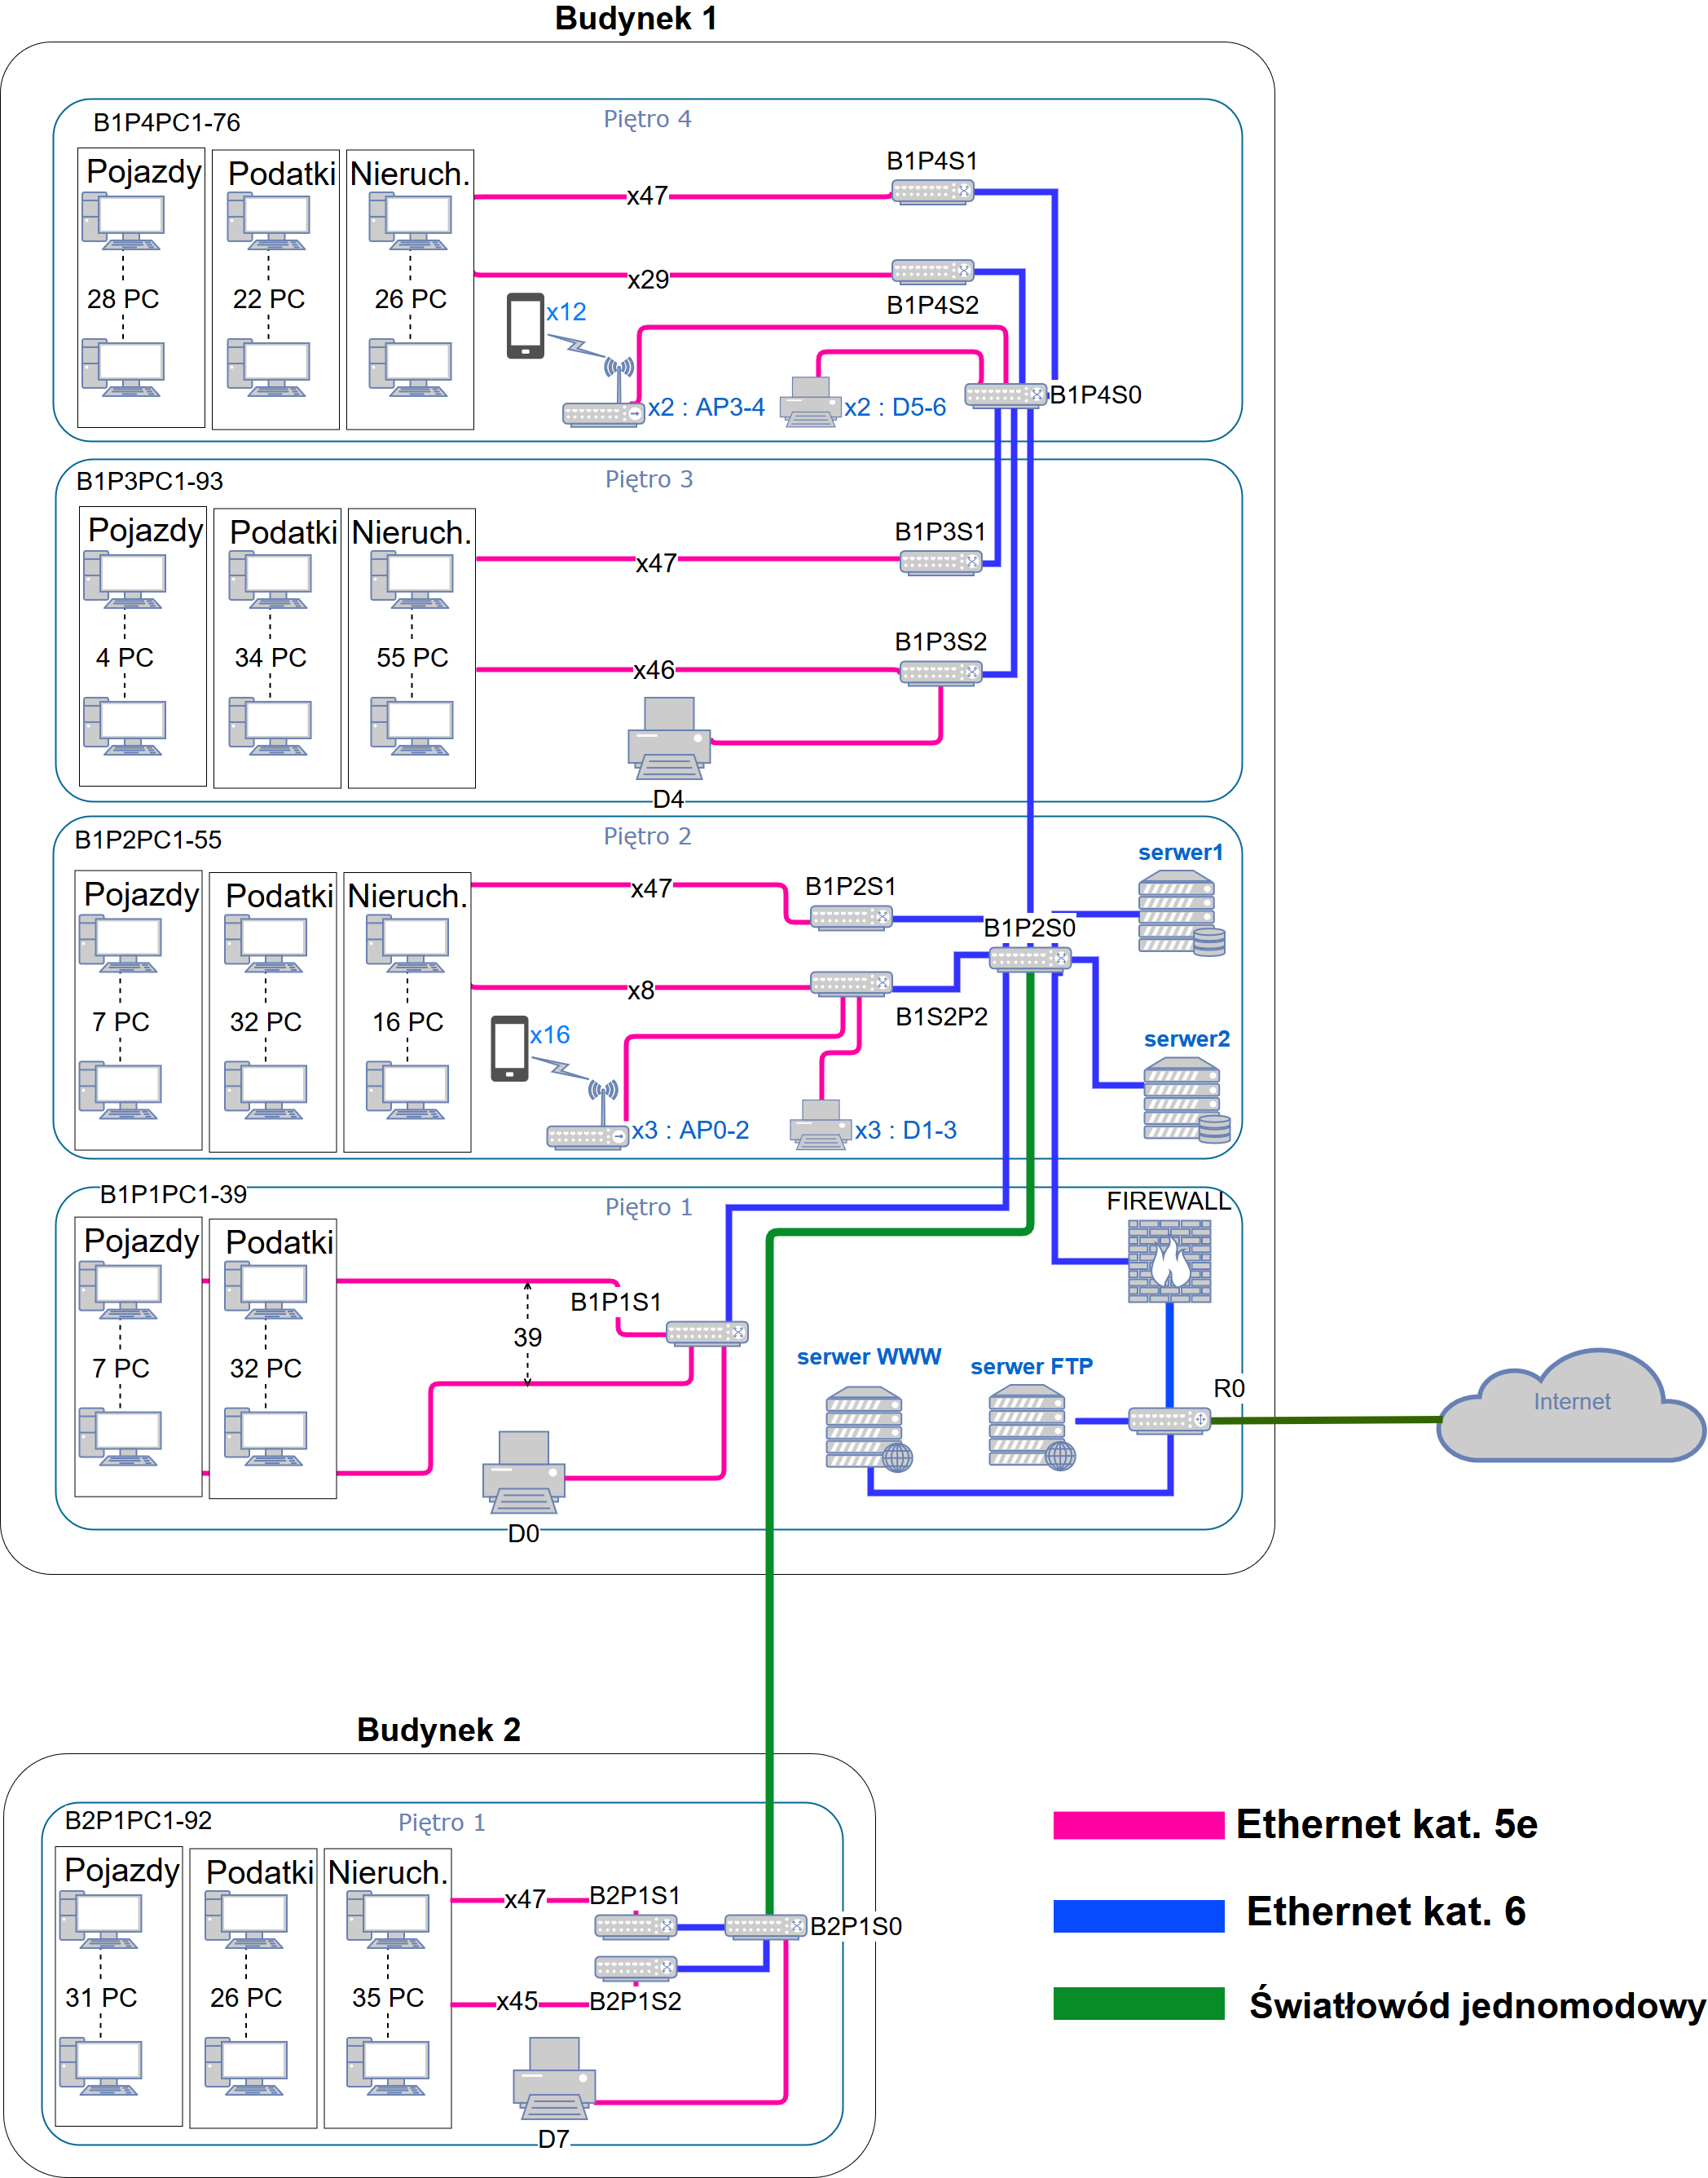
\includegraphics[width = \textwidth]{obrazki/diag.png}
	    \caption{Projekt logiczny sieci}
	    \label{fig:projekt}
	\end{figure}
	    
	\subsection{Wybór urządzeń sieciowych}
	
	\begin{itemize}
		\item Router - Cisco 4451-X
		\item Firewall - Cisco Firepower 2110
		\item Switche - Cisco Catalyst WS-C3650-24TS x2
		\item Switche - Cisco Catalyst C9300-48T x8
		\item Switche SFP (B1P2S0, B2P1S0)- Cisco SG350-10SFP x2
		\item Punkty dostępowe wifi - Access Point Cisco Aironet 2702I-E-K9 x5
	\end{itemize}

	\subsection{Projekt adresacji IP}
	
		\begin{figure}[H]
			\centerin
			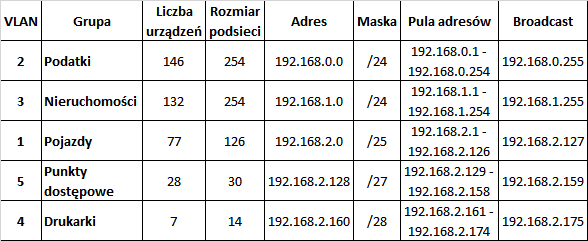
\includegraphics[width = \textwidth]{obrazki/vlany.png}
			\caption{Adresacja sieci}
			\label{fig:vlany}
		\end{figure}
	    
	\subsection{Projekt konfiguracji urządzeń}
	
	\subsection{Projekt podłączenia do Internetu}
	
	\subsection{Kosztorys}
	
	\section{Karty katalogowe proponowanych urządzeń}
	
	\begin{itemize}
		\item Cisco ASR 1002-X - https://www.cisco.com/c/en/us/support/routers/asr-1002-x-router/model.html
		\item Cisco Firepower 2110 - https://www.cisco.com/c/en/us/support/security/firepower-2110-security-appliance/model.html
		\item Cisco Catalyst C9200-48P - https://www.cisco.com/c/en/us/support/switches/catalyst-9200-48p-4g-switch/model.html
		\item Cisco Catalyst C9300-48T - https://www.cisco.com/c/en/us/support/switches/catalyst-9300-48t-a-switch/model.html
		\item Cisco SG350-10SFP - https://www.cisco.com/c/en/us/support/switches/sg350-10sfp-10-port-gigabit-managed-sfp-switch/model.html
	\end{itemize}
	
\end{document}